\chapter{Ярость против конечных автоматов}
\label{rage-against-the-finite-state-machines}
\section{Кто они такие?}
\label{what-are-they}
Конечные автоматы (КА) не имеют ничего общего с огнестрельным оружием.
Их главным признаком является наличие конечного числа состояний.
Мне всегда было проще понимать конечные автоматы, если они изображены в виде графиков и диаграмм.
К примеру, такая нехитрая диаграмма описывает (очень глупую) собаку в виде автомата состояний.
\begin{figure}[h!]
    \centering
    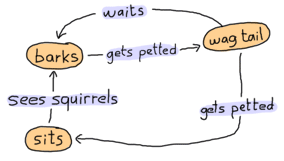
\includegraphics[width=0.7\textwidth]{fsm_dog.png}
\end{figure}
Собака может находиться в трёх состояниях: она может сидеть, гавкать или вилять хвостом.
Различные события или входные цепочки могут вынудить её поменять состояние.
Если собака спокойно сидит и видит белку, она начнёт гавкать и не остановится, пока её не погладят.
Но если собака сидит и вы её погладите, мы даже представить не в состоянии, что может произойти.
В мире Erlang собака сможет аварийно завершиться (и, в конце концов, её перезапустит супервизор).
В реальности такое событие выглядело бы очень странно: ваша собака, после того как её задавила машина, смогла бы просто ожить, что, в принципе, не так уж и плохо.

Для сравнения я приведу диаграмму состояний кошки:

\begin{figure}[h!]
    \centering
    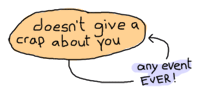
\includegraphics[width=0.7\textwidth]{fsm_cat.png}
\end{figure}

Эта кошка всегда находится в одном и том же состоянии, и никакое событие никогда не сможет его изменить.

\href{http://learnyousomeerlang.com/static/erlang/cat\_fsm.erl}{Автомат, который описывает состояния кошки}, можно легко и просто реализовать на Erlang:
\begin{lstlisting}[style=erlang]
-module(cat_fsm).
-export([start/0, event/2]).
 
start() ->
    spawn(fun() -> dont_give_crap() end).
 
event(Pid, Event) ->
    Ref = make_ref(), % won't care for monitors here
    Pid ! {self(), Ref, Event},
    receive
        {Ref, Msg} -> {ok, Msg}
    after 5000 ->
        {error, timeout}
    end.
 
dont_give_crap() ->
    receive
        {Pid, Ref, _Msg} -> Pid ! {Ref, meh};
        _ -> ok
    end,
    io:format("Switching to 'dont_give_crap' state~n"),
    dont_give_crap().
\end{lstlisting}
Мы можем попробовать модуль в деле, чтобы убедиться, что кошка всегда сохраняет невозмутимость:
\begin{lstlisting}[style=erlang]
1> c(cat_fsm).
{ok,cat_fsm}
2> Cat = cat_fsm:start().
<0.67.0>
3> cat_fsm:event(Cat, pet).
Switching to 'dont_give_crap' state
{ok,meh}
4> cat_fsm:event(Cat, love).
Switching to 'dont_give_crap' state
{ok,meh}
5> cat_fsm:event(Cat, cherish).
Switching to 'dont_give_crap' state
{ok,meh}
\end{lstlisting}
То же самое можно сделать и для \href{http://learnyousomeerlang.com/static/erlang/dog\_fsm.erl}{конечного автомата, который описывает поведение собаки}.
В отличие от кошки, собаке доступно большее количество состояний:
\begin{lstlisting}[style=erlang]
-module(dog_fsm).
-export([start/0, squirrel/1, pet/1]).
 
start() ->
    spawn(fun() -> bark() end).
 
squirrel(Pid) -> Pid ! squirrel.
 
pet(Pid) -> Pid ! pet.
 
bark() ->
    io:format("Dog says: BARK! BARK!~n"),
    receive
        pet ->
            wag_tail();
        _ ->
            io:format("Dog is confused~n"),
            bark()
    after 2000 ->
        bark()
    end.
 
wag_tail() ->
    io:format("Dog wags its tail~n"),
    receive
        pet ->
            sit();
        _ ->
            io:format("Dog is confused~n"),
            wag_tail()
    after 30000 ->
        bark()
    end.
 
sit() ->
    io:format("Dog is sitting. Gooooood boy!~n"),
    receive
        squirrel ->
            bark();
        _ ->
            io:format("Dog is confused~n"),
            sit()
    end.
\end{lstlisting}
Мы сможем относительно легко установить соответствие между каждым состоянием, переходом, и тем, что было изображено на диаграмме.
Вот как выглядит конечный автомат в деле:
\begin{lstlisting}[style=erlang]
6> c(dog_fsm).
{ok,dog_fsm}
7> Pid = dog_fsm:start().
Dog says: BARK! BARK!
<0.46.0>
Dog says: BARK! BARK!
Dog says: BARK! BARK!
Dog says: BARK! BARK!
8> dog_fsm:pet(Pid).
pet
Dog wags its tail
9> dog_fsm:pet(Pid).
Dog is sitting. Gooooood boy!
pet
10> dog_fsm:pet(Pid).
Dog is confused
pet
Dog is sitting. Gooooood boy!
11> dog_fsm:squirrel(Pid).
Dog says: BARK! BARK!
squirrel
Dog says: BARK! BARK!   
12> dog_fsm:pet(Pid).
Dog wags its tail
pet
13> %% wait 30 seconds
Dog says: BARK! BARK!
Dog says: BARK! BARK!
Dog says: BARK! BARK!    
13> dog_fsm:pet(Pid).    
Dog wags its tail
pet
14> dog_fsm:pet(Pid).
Dog is sitting. Gooooood boy!
pet
\end{lstlisting}

Можете, если хотите, отслеживать состояния по схеме (я обычно так и делаю \--- это помогает убедиться, что всё сделано верно).

Вот так и выглядит основа конечного автомата, реализованного при помощи процессов Erlang.
Мы могли бы кое\--что сделать иначе: можно передавать состояние в аргументах функций состояния.
Что\--то похожее мы делаем в реализации главного цикла сервера.
Также мы могли бы добавить функции \ops{init} и \ops{terminate}, обработку обновления кода и т.п.

Есть и ещё одно отличие между конечными автоматами собаки и кошки \--- кошка использует \emph{синхронные} события, а собака \emph{асинхронные}.
В реальном конечном автомате можно было бы использовать и тот и другой вид событий, но из\--за чистой незамутнённой лени, я выбрал самое простое представление из возможных.
Также существует ещё один вид событий, не показанный в примерах \--- это глобальные события, которые могут возникать в любом состоянии.

Примером такого события может стать факт "собака учуяла еду".
Как только сработает событие \ops{smell\_food}, пёс начнёт искать источник запаха, в каком бы состоянии он не находился. 

Но не будем долго задерживаться на реализации всего перечисленного в нашем грубом наброске конечного автомата.
Лучше перейдём прямо к стратегии поведения \ops{gen\_fsm}.
\section{Обобщённые конечные автоматы}
\label{generic-finite-state-machines}
Стратегия поведения \ops{gen\_fsm} схожа с \ops{gen\_server} тем, что она является её специализированной разновидностью.
Главное отличие gen\_fsm заключается в том, что вместо обработки \emph{вызовов (calls)} и \emph{cast-запросов (casts)} мы обрабатываем \emph{синхронные} и \emph{асинхронные события}.
Каждое состояние, как и в наших примерах с кошкой и собакой, будет представлено функцией.
Мы снова перечислим функции обратного вызова, которые должны быть реализованы нашими модулями для корректной работы.
\subsection{init}
\label{init2}
Это тот же самый \href{http://erldocs.com/R15B/stdlib/gen\_fsm.html\#init/1}{init/1}, который используется в серверах общего назначения, но с несколькими отличиями: он принимает в качестве возвращаемых значений кортежи \ops{\{ok, StateName, Data\}}, \ops{\{ok, StateName, Data, Timeout\}}, \ops{\{ok, StateName, Data, hibernate\}} и \ops{\{stop, Reason\}}.
Кортеж с атомом \ops{stop} работает так же как в \ops{gen\_server}\--ах.
Та же семантика сохраняется и для \ops{hibernate} с \emph{Timeout}.

Новизна скрывается в переменной \emph{StateName}.
\emph{StateName} это атом, определяющий очередную функцию обратного вызова, которую необходимо вызвать.
\subsection{StateName}
\label{statename}
\begin{wrapfigure}{r}{0.35\linewidth}
    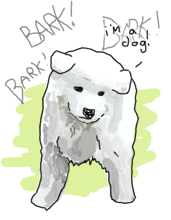
\includegraphics[width=1\linewidth]{dog.png}
\end{wrapfigure}
Имена функций \href{http://erldocs.com/R15B/stdlib/gen\_fsm.html\#StateName/2}{StateName/2} и \href{http://erldocs.com/R15B/stdlib/gen\_fsm.html\#StateName/2}{StateName/3} определяютkkвы должны заменить на те, которые посчитаете нужными.
Предположим, что функция \ops{init/1} возвращает кортеж \ops{\{ok, sitting, dog\}}.
Значит, конечный автомат находится в состоянии \ops{sitting}.
Это не тот же самый вид состояния, который мы видели в \ops{gen\_server}, его можно назвать эквивалентом для состояний \ops{sit}, \ops{bark} и \ops{wag\_tail} предыдущего конечного автомата, описывающего поведение собаки.
Эти состояния задают контекст, в котором вы обрабатываете заданное событие.

Как пример можно привести ситуацию, когда кто\--либо звонит вам по телефону.
Если ваше текущее состояние <<сон субботним утром>>, то на звонок вы, должно быть, отреагируете криками в телефонную трубку.
Если ваше состояние <<ожидаю собеседования>>, то вы, скорее всего, вежливо ответите на звонок.
Ну и если вы пребываете в состоянии <<умер>>, то мне не вполне ясно как вы вообще смогли прочитать эти строки.

Вернёмся к нашему конечному автомату.
Функция \ops{init/1} сообщила, что мы должны находиться в состоянии \ops{sitting}.
Всякий раз когда процесс \ops{gen\_fsm} принимает уведомление о событии, будет вызвана либо функция \ops{sitting/2}, либо \ops{sitting/3}.
Функция \ops{sitting/2} вызывается для асинхронных событий, а \ops{sitting/3} для синхронных.

Аргументами для \ops{sitting/3} будут \emph{Event}, само сообщение, переданное в качестве события, и \emph{StateData}: данные, которые передавались от вызова к вызову.
Функция \ops{sitting/2} может возвратить кортежи \ops{\{next\_state, NextStateName, NewStateData\}}, \ops{\{next\_state, NextStateName, NewStateData, Timeout\}}, \ops{\{next\_state, NextStateName, hibernate\}} и \ops{\{stop, Reason, NewStateData\}}.

Для \ops{sitting/3} передаются похожие аргументы, только между \emph{Event} и \emph{StateData} передаётся переменная \emph{From}.
Переменная \emph{From} используется совершенно так же как она использовалась в \ops{gen\_server}\--ах, включая \href{http://erldocs.com/R15B/stdlib/gen\_fsm.html\#reply/2}{gen\_fsm:reply/2}.
Функции \ops{StateName/3} могут возвращать следующие кортежи:
\begin{lstlisting}[style=erlang]
{reply, Reply, NextStateName, NewStateData}
{reply, Reply, NextStateName, NewStateData, Timeout}
{reply, Reply, NextStateName, NewStateData, hibernate}

{next_state, NextStateName, NewStateData}
{next_state, NextStateName, NewStateData, Timeout}
{next_state, NextStateName, NewStateData, hibernate}

{stop, Reason, Reply, NewStateData}
{stop, Reason, NewStateData}
\end{lstlisting}

Обратите внимание, что количество этих функций никак не ограничивается, но лишь при условии, что они проэкспортированы.
Атомы, возвращаемые в кортежах как \emph{NextStateName}, определяют, будет ли функция вызвана или нет.

\subsection{handle\_event}
\label{handle-event}
В предыдущем разделе я упомянул о глобальных событиях, которые могут спровоцировать определённую реакцию, не зависящую от нашего текущего состояния (собака, которая учуяла пищу, бросит своё текущее занятие, и приступит к поиску еды).
Для событий, которые необходимо обрабатывать одинаково в каждом состоянии, лучше всего подойдёт функция обратного вызова (callback) \href{http://erldocs.com/R15B/stdlib/gen\_fsm.html\#handle\_event/3}{handle\_event/3}.
Список аргументов для этой функции похож на \ops{StateName/2}, за исключением дополнительной переменной \emph{StateName}, которая указывает, каким было состояние в момент получения события.
Возвращает она те же значения, что и \ops{StateName/2}.
\subsection{handle\_sync\_event}
\label{handle-sync-event}
Функция обратного вызова \href{http://erldocs.com/R15B/stdlib/gen\_fsm.html\#handle\_sync\_event/4}{handle\_sync\_event/4} относится к \ops{StateName/3} так же, как \ops{handle\_event/2} относится к \ops{StateName/2}.
Она обрабатывает синхронные глобальные события, принимает те же самые параметры и возвращает кортежи того же вида, что и \ops{StateName/3}.

Настал подходящий момент для объяснения принципа, по которому мы определяем, относиться ли событие к глобальным или его необходимо отсылать к определённому состоянию.
Для этого мы можем взглянуть на функцию, которая используется для отсылки события к КА (конечному автомату).
Асинхронные события предназначенные для любой функции \ops{StateName/2} отправляются при помощи \href{http://erldocs.com/R15B/stdlib/gen\_fsm.html\#send\_event/2}{send\_event/2}, а синхронные события, которые должны обрабатываться \ops{StateName/3} отсылаются \href{http://erldocs.com/R15B/stdlib/gen\_fsm.html\#sync\_send\_event/2}{sync\_send\_event/2-3}.

Для глобальных событий двумя эквивалентными функциями являются \href{http://erldocs.com/R15B/stdlib/gen\_fsm.html\#send\_all\_state\_event/2}{send\_all\_state\_event/2} и \href{http://erldocs.com/R15B/stdlib/gen\_fsm.html\#sync\_send\_all\_state\_event/2}{sync\_send\_all\_state\_event/2-3} (весьма длинное имя).

\subsection{code\_change}
\label{code-change}
Эта функция работает совершенно так же как и для \ops{gen\_server}\--а, за исключением того, что она принимает дополнительный переметр состояния при вызове \ops{code\_change(OldVersion, StateName, Data, Extra)} и возвращает кортеж вида \ops{\{ok, NextStateName, NewStateData\}}.

\subsection{terminate}
\label{terminate}
Эта функция, опять же, действует приблизительно так же как и для обобщенных серверов.
Функция \href{http://erldocs.com/R15B/stdlib/gen\_fsm.html\#terminate/3}{terminate/3} должна выполнять действия, противоположные тем, которые выполняются в \ops{init/1}.
